\section{Búsqueda de vacantes de oxígeno en STO mediante imágenes 4D-STEM}

\begin{wrapfigure}{o}{6.5cm}
    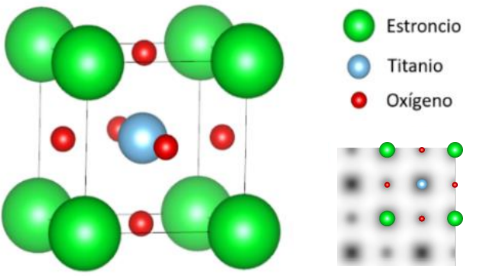
\includegraphics[width=0.38\textwidth]{fig/Fig15.png}
    \caption{En esta imagen se muestra un esquema de la celda unidad de SrTiO$_3$ (STO), junto a su visualización sobre una imagen simulada ABF \cite{paquito}.}
    \label{fig:15}
\end{wrapfigure} 

% Introducción con información física sobre las vacantes de oxígeno en STO y cómo están ligadas a las propiedades del material. ¿Para qué se usa STO?

Bla blaBla blaBla blaBla blaBla blaBla blaBla blaBla blaBla blaBla blaBla blaBla blaBla blaBla blaBla blaBla blaBla blaBla blaBla blaBla blaBla blaBla blaBla blaBla blaBla blaBla blaBla blaBla blaBla blaBla blaBla blaBla blaBla blaBla blaBla blaBla blaBla blaBla blaBla blaBla blaBla blaBla blaBla blaBla blaBla blaBla blaBla blaBla blaBla blaBla blaBla blaBla blaBla blaBla blaBla blaBla blaBla blaBla blaBla blaBla blaBla blaBla blaBla blaBla blaBla blaBla blaBla blaBla blaBla blaBla blaBla blaBla blaBla blaBla blaBla blaBla blaBla blaBla blaBla blaBla aBla blaBla blaBla blaBlaaBla blaBla blaBla blaBlaaBla blaBla blaBla blaBla aBla blaBla blaBla blaBla blaBla blaBla blaBla blaBla blaBla blaBla blaBla aBla blaBla blaBla blaBlaaBla blaBla blaBla blaBlaaBla blaBla blaBla blaBla aBla blaBla blaBla blaBla 



\newpage
\subsection{Procesamiento de imágenes ABF de STO}

Partiendo de la imagen ABF que se muestra en la \autoref{fig:16}, llevaremos a cabo varios procesos de \textit{denoising}. Nuestro objetivo principal es sacar a la luz las columnas de oxígeno que, según se muestra en la simulación de la \autoref{fig:15}, deberían de poder apreciarse sin problemas sobre la región de integración del patrón de difracción en la que estamos trabajando.

\begin{figure}[h!]
    \centering
    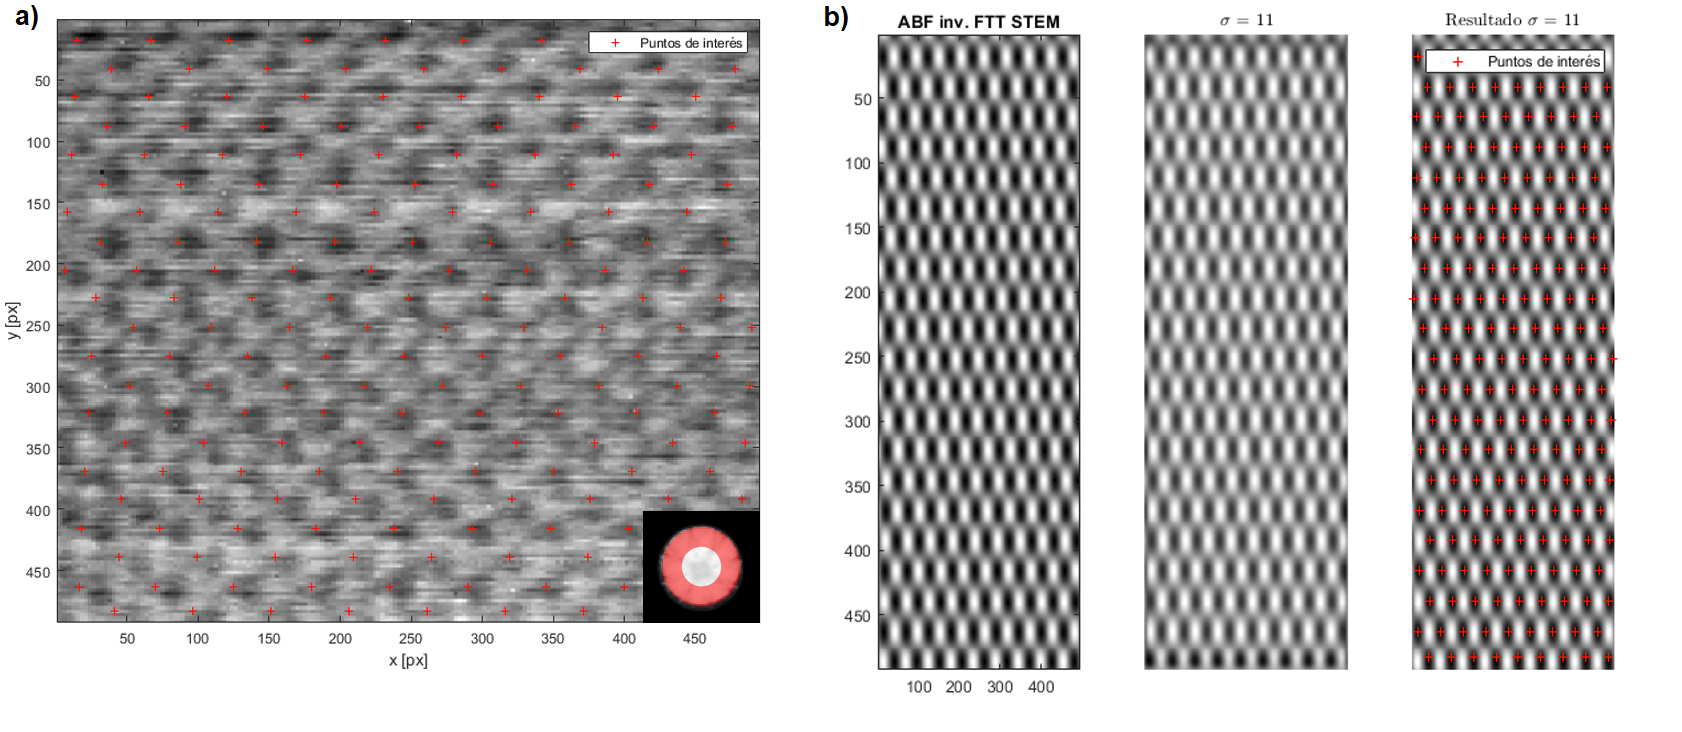
\includegraphics[width=1\textwidth]{fig/Fig16.png}
    \caption{\textbf{a)} Imagen ABF tomada por Francisco Fernández Cañizares sobre una muestra de STO horneada a 500 ºC durante 8 h - 6C 10cm df0. En la esquina inferior derecha aparece la región de integración sobre el patrón de difracción (15:30 mrads) seleccionada para generar dicha imagen. Los puntos de interés han sido escogidos por el algoritmo de detección de \textit{blobs}, cuyo \textit{input} corresponde con \textbf{b)} un filtrado FFT de alto umbral sobre la imagen ABF invertida. Programa desarrollado en MATLAB por el autor \cite{repo}.}
    \label{fig:16}
\end{figure}

\subsubsection{Generación de parches con información sobre la celda unidad}

La entrada para los distintos algoritmos de \textit{denoising} será un \textit{stack} de parches (ver Figura \ref{fig:17}a) que únicamente van a contener información sobre la celda unidad STO. Para llevar a cabo esta selección, inicialmente aplicaremos un PCA a los parches generados entorno a todos los puntos de interés. Esto nos permitirá filtrar en función de la primera componente principal aquellos parches que corresponden a columnas de Ti.\\

\subsubsection{\textit{Denoising} por PCA y NMF}
Una vez hemos generado el \textit{clean stack} de celdas unidad, volvemos a aplicar PCA y NMF (Figura \ref{fig:17}c), esta vez para realizar un promedio que nos permita extraer la información común entre todas las imágenes del \textit{stack}.

% Discusión: ¿Qué estamos observando? ¿Son buenos resultados?

\newpage

\begin{figure}[h!]
    \centering
    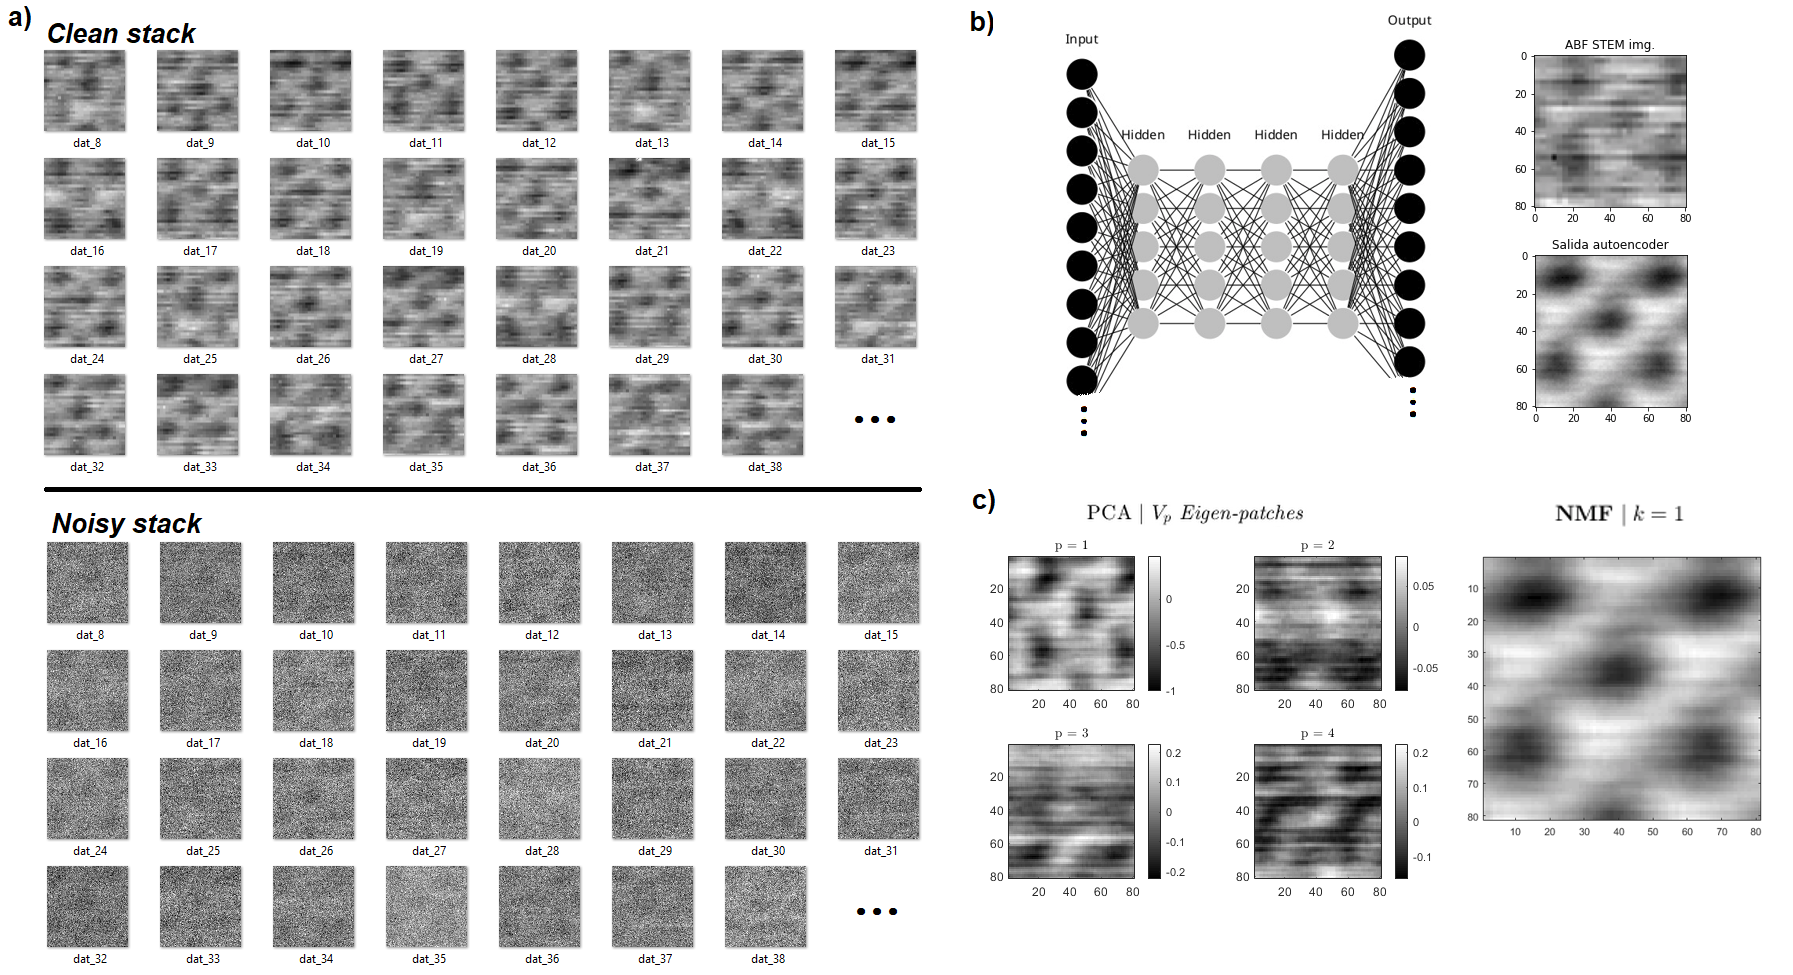
\includegraphics[width=1\textwidth]{fig/Fig17.png}
    \caption{ \cite{repo}.}
    \label{fig:17}
\end{figure}

\subsubsection{\textit{Denoising} por una red con topología de \textit{autoencoder}}



% Discusión: ¿Qué estamos observando? ¿Son buenos resultados?



